\section{实验:用滑动变阻器改变电流强度}\label{sec:8-11}

在这个实验里我们练习使用滑动变阻器。
实验室里的滑动变阻器,多数是图 \ref{fig:8-19} 所示的那样有四个接线柱,使用时要注意防止接错。
使用前观察滑动变阻器上标的电阻值和允许通过的最大电流值。
使用时注意通过变阻器的电流强度不要超过允许的最大值。

照图 \ref{fig:8-22} 将电池组、安培表、5 欧姆的定值电阻 $R$(或其他阻值的)、伏特表、电键连接起来,
$M$、$N$ 两个线头暂时不接,准备接入滑动变阻器 $R'$。

\begin{figure}[htbp]
    \centering
    \begin{minipage}{7cm}
    \centering
    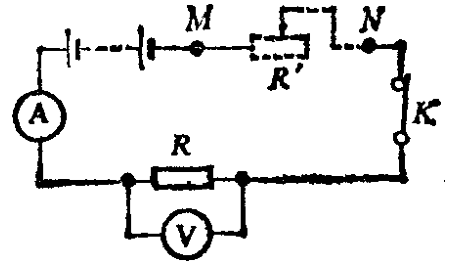
\includegraphics[width=6cm]{../pic/czwl2-ch8-22}
    \caption{}\label{fig:8-22}
    \end{minipage}
    \qquad
    \begin{minipage}{7cm}
    \centering
    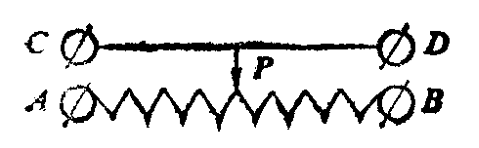
\includegraphics[width=6cm]{../pic/czwl2-ch8-23}
    \caption{}\label{fig:8-23}
    \end{minipage}
\end{figure}

象图 \ref{fig:8-23} 那样,用 $A$、$B$、$C$、$D$ 分别代表滑动变阻器的四个接线柱。
先将线头 $M$、$N$ 分别接到 $A$、$C$ 上,移动滑片 $P$,观察安培表指针。
看 $P$ 向哪个方向滑动时电流减小,向哪个方向滑动时电流增大。想想看,为什么?
再将 $M$、$N$ 分别接到 $A$、$D$ 上,重复上述的实验。
对这两种接法各画一个变阻器的结构示意图,在图上用红铅笔画出电流通过变阻器的路径。

想想看,为了使变阻器能改变电路中的电流,还可以有哪两种接法。
对这两种接法各画一个变阻器的结构示意图,标明电流路径,并且想清滑片移动方向跟电流变化的关系,
然后将变阻器接入电路,检查自己的想法是否正确。

调节滑片 $P$ 的位置,观察电流强度分别为 0.1、0.2、0.3 安培时 $R$ 两端的电压值,
将这三组数据记在下面的表格里。

\jiange
\begin{tblr}{
    hlines, vlines,
    colspec={ccccc},
    column{3-5}={wd=4em},
    %cells={valign=m},
}
    \SetCell[r=2]{c} $R=5$欧姆 & $I$(安培)& 0.1 & 0.2 & 0.3 \\
    & $U$(伏特) & & & \\
\end{tblr}
\jiange

根据表里的数据回答:利用滑动变阻器使某部分电路(电阻 $R$)中的电流增大或减小时,
这部分电路两端的电压怎样改变?

如果把线头 $M$、$N$ 分别接到 $A$、$B$ 两个接线柱上,或者分别接到 $C$、$D$ 两个接线柱上,
移动滑片 $P$,安培表的示数改变吗?用实验检查你的答案是否正确。


\lianxi

(1) 有两条同样粗细的导线,是同一种材料做成的。
一条长 20 厘米,另一条长 1.3 米。哪一条电阻大,为什么?

(2) 有两条同样长短的导线,是同一种材料做成的。
一条的截面积是 0.4 $\pflm$, 另一条是 2 $\pfhm$。哪一条电阻大,为什么?

(3) 图 \ref{fig:8-24} 画了四个滑动变阻器的结构示意图,并且表示出了它们连入电路的情形。
对每个变阻器分别说明:滑片向左动时和向右动时,连入电路的电阻怎样改变?
电路中的电强度怎样改变?

\begin{figure}[htbp]
    \centering
    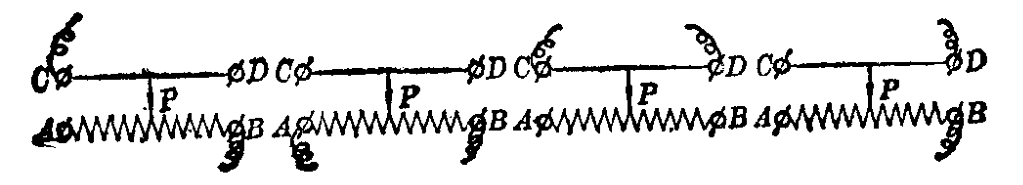
\includegraphics[width=0.8\textwidth]{../pic/czwl2-ch8-24}
    \caption{}\label{fig:8-24}
\end{figure}

(4) 图 \ref{fig:8-25} 表示的是一种自动测定油箱内油面高度的装置。
$R$ 是滑动变阻器,它的金属滑片是杠杆的一端,从油量表(电流表)指针所指的刻度,
就可以知道油箱内油面的高度。说明它的工作原理。

\begin{figure}[htbp]
    \centering
    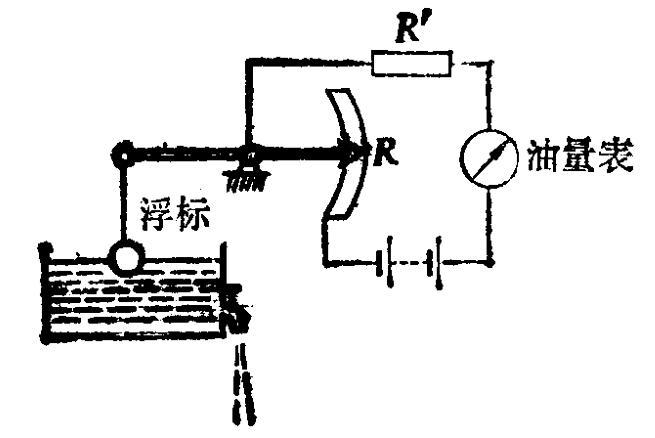
\includegraphics[width=0.6\textwidth]{../pic/czwl2-ch8-25}
    \caption{}\label{fig:8-25}
\end{figure}


\section*{小实验}

在这个小实验里,我们自己做一个滑动变阻器,并且用它来控制小灯泡的亮度。

首先用小木板、图钉、薄铁片、细铜丝(或细铁丝)、小木夹等,
按照图 \ref{fig:8-26} 中所画的样子制做一个电池夹和一只小灯座。

\begin{figure}[htbp]
    \centering
    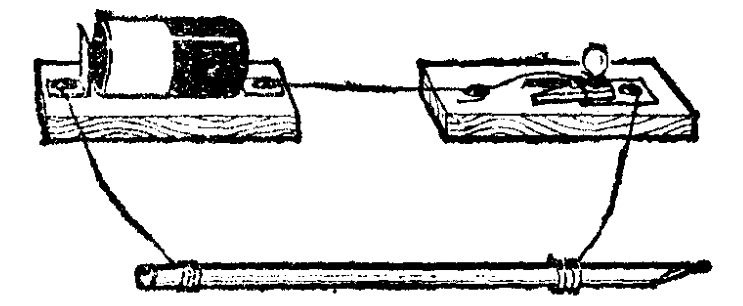
\includegraphics[width=0.6\textwidth]{../pic/czwl2-ch8-26}
    \caption{}\label{fig:8-26}
\end{figure}

然后用小刀将铅笔剖成两半,留下附着铅笔心的那一半。
在铅笔心的一端接一根导线(用细线绑紧或用胶布粘住)。
找一小段铜线,在铅笔上绕几圈,做成一个能在铅笔上滑动的铜坏。
这样就做成了一个滑动变阻器。

最后,参照图 \ref{fig:8-26} 用导线把电池、小灯泡和自制的变阻器连接起来,
观察铜环在铅笔上滑动时小灯泡亮度的变化。

注意:在用一节干电池的情况下,要选用标着 1.2 V 的小灯泡。

